\documentclass[conference]{IEEEtran}

\usepackage[utf8]{inputenc}
\usepackage[T1]{fontenc}
\usepackage[english]{babel}
\usepackage{graphicx}
\graphicspath{{main_2_images/}{Tecnologia_en_Marcha/main_2_images/}}
\usepackage{array}
\usepackage{tabularx}
\usepackage{url}
\usepackage{cite}

\urlstyle{same}

\title{Digitalization of Community-Managed Rural Aqueducts in Costa Rica}

\author{
\IEEEauthorblockN{María José Angulo Campos}
\IEEEauthorblockA{
\textit{Tecnológico de Costa Rica}\\
Cartago, Costa Rica \\
https://orcid.org/0009-0005-5842-1101}
\and
\IEEEauthorblockN{Carlos Montoya Marín}
\IEEEauthorblockA{
\textit{Tecnológico de Costa Rica}\\
Cartago, Costa Rica \\
https://orcid.org/0009-0001-1561-9768}
\and
\IEEEauthorblockN{Juan José Montero-Jiménez}
\IEEEauthorblockA{
\textit{Tecnológico de Costa Rica}\\
Cartago, Costa Rica \\
https://orcid.org/0000-0002-3215-3736}
\and
\IEEEauthorblockN{Juan José Rojas-Hernández}
\IEEEauthorblockA{
\textit{Tecnológico de Costa Rica}\\
Cartago, Costa Rica \\
https://orcid.org/0000-0002-3261-5005}
}

\begin{document}
\maketitle

\begin{abstract}
This article synthesizes the development trajectory of digital monitoring solutions for Costa Rican ASADAS and derives architectural criteria for adaptation to other sites. The analysis uses a comparative case synthesis of Las Juntas de Abangares, Playa Sámara, and Paso Ancho--Boquerón, considering the operational problem, requirements, design process, measured variables, interfaces, energy, communication, digital services, evidence, and limitations. The findings are organized according to the MBSE distinction between needs, logical functions, and physical implementation. The synthesis identifies a stable functional core---remote observability, interoperability with existing assets, fewer required site visits, energy autonomy, decision support, and maintainability---that can be implemented through a modular chain of measurement, acquisition, communication, storage, visualization, and alerting. The prototypes provide partial and incremental technical evidence, and the current Paso Ancho design is an instantiation still under development. This article reports no new field validation or measured effects on losses, continuity, workload, or costs. Assessing these effects requires sustained operation.
\end{abstract}

\begin{IEEEkeywords}
rural aqueducts, community-managed water systems, ASADA, Internet of Things, remote monitoring, Model-Based Systems Engineering, modular architecture
\end{IEEEkeywords}

\section{Introduction}
Digital transformation in water infrastructure integrates sensing, communications, data management, and automation within an operational system \cite{arnell2023making,zulkifli2022iot,velayudhan2022iot}. This integration is especially important in rural aqueducts, where assets are dispersed and access to personnel, maintenance, energy, and connectivity may be limited. In Costa Rica, more than 2000 community water organizations, or ASADAS, operate these systems \cite{direccion2025asadas}, and previous studies have documented constraints in infrastructure, maintenance, and technical capacity \cite{soto2016situacion,gaviria2020risk}.

Digitalizing a rural aqueduct requires adapting sensing and data services to limited energy, intermittent connectivity, existing instrumentation, manual routines, and information needs for supply planning. The engineering challenge is to convert dispersed measurements into reliable, accessible, and useful operational information.

This article synthesizes three prototyping experiences in Costa Rican ASADAS. Las Juntas de Abangares moved from discrete manual measurement to autonomous level acquisition, cellular communication, storage, and visualization \cite{chavarria2021implementacion}. Playa Sámara expanded the scope to distributed monitoring, LoRa links, IoT services, alarms, and control-oriented design \cite{solorzano2021sistema}. Paso Ancho--Boquerón explored industrial interfaces, Modbus, 4--20~mA sensing, remote telemetry, and replicability \cite{oviedo2024desarrollo}. Part of this learning was later formalized as a modular architecture through MBSE \cite{arguedas2025towards}.

The scope is delimited with respect to the ISSE 2025 paper, which focuses on a generic and modular architecture for IoT systems in rural aqueducts using ARCADIA/MBSE \cite{arguedas2025towards}. This manuscript reconstructs the preceding technical trajectory, includes Las Juntas de Abangares, and compares prototype evidence, generalized capabilities, and current design decisions.

The contributions are:
\begin{enumerate}
\item To compare the requirements, design processes, implementations, and test evidence of three ASADA digitalization developments.
\item To identify recurring operational needs and architectural implications.
\item To distinguish tested functions, MBSE-formalized capabilities, and current Paso Ancho elements that remain subject to deployment.
\item To propose criteria for transferability and evaluation within the limits of the available evidence.
\end{enumerate}

\section{Method}
We used a qualitative comparative case synthesis to integrate heterogeneous prototype evidence. The cases were selected because they form a documented sequence from Laboratorio Delta/TEC with Costa Rican ASADAS, cover tank-level acquisition, distributed monitoring with existing meters, and industrial interfaces, and have available technical sources. The sample is limited to these three developments.

The primary sources were the technical reports and final graduation projects for Las Juntas de Abangares, Playa Sámara, and Paso Ancho--Boquerón \cite{chavarria2021implementacion,solorzano2021sistema,oviedo2024desarrollo}. The same extraction categories were applied to each report:
\begin{enumerate}
\item Operational problem and requirements, including user needs, existing assets, and site constraints.
\item Design process, including functional decomposition, alternatives considered, selection criteria, integration steps, and revisions prompted by tests.
\item Implementation, including hydraulic variables, sensors and interfaces, controller, energy supply, communication, and digital services.
\item Evidence and limits, including the function tested, test setting, reference measurement, reported result, and pending verification.
\end{enumerate}
The case descriptions follow this order and cite the sections that document the design decisions and tests. Details absent from a source were left unreported. The comparison preserves differences in the methods used by the original authors.

Two complementary sources served distinct purposes. The ISSE 2025 paper provided the published ARCADIA/MBSE architecture used to interpret the cases \cite{arguedas2025towards}. For the current Paso Ancho application, the firmware, requirements, bill of materials, functional-version document, and integration, verification, and validation plan were analyzed \cite{deltalabo2026repo}. Findings about this application are limited to that version and document design and planned integration. Field performance remains to be established.

A need was classified as recurring when the same operational purpose appeared in at least two cases. Requirements specific to one case were retained as site constraints, and additional capabilities from the MBSE architecture were identified separately. The synthesis then related these needs to capabilities, logical functions, and physical implementations.

For each function, the extraction distinguished implementation status from verification evidence: bench or laboratory tests, limited field tests, reported sustained operation, calculations or simulations, and planned verification. Table~\ref{tab:cases} summarizes the evidence for the three prototypes. The term LoRa describes the documented long-range radio links. The original reports' use of LoRaWAN is noted where relevant, with the network interpretation limited to the documented gateway and packet handling. This study produced a technical synthesis and design criteria. It involved no new measurements, prolonged trials, or statistical analyses of water losses.

\section{Recurring Digitalization Needs}
Recurring operational needs emerged from user requirements, site constraints, sensor tests, energy estimates, and communication and visualization decisions across the three experiences. Table~\ref{tab:needs} summarizes their relationship with architectural decisions.

\subsection{From Manual Measurements to Remote Observability}
The first need was to turn intermittent records into remote observability. In Las Juntas de Abangares, tank level was measured approximately every fifteen days with a scale and recorded in a notebook, which prevented observation of daily or seasonal variations and modeling of demand and supply \cite{chavarria2021implementacion}. The prototype tested automatic measurements every hour or every 20 minutes, including date and time stamps, plots, and data download. These functions made records available for remote consultation. Their performance during sustained operation remains unreported.

Sámara and Paso Ancho--Boquerón expanded monitoring beyond tank level and incorporated variables such as flow, volume, communication status, and operating conditions \cite{solorzano2021sistema,oviedo2024desarrollo}. This shows that a single measurement is not sufficient to understand how the aqueduct operates. To support decision-making, the system must integrate several measurements that describe the hydraulic and operational state with adequate frequency and reliability.

\subsection{Interoperability with Existing Infrastructure}
ASADAS do not start from the same technological baseline: some have usable meters, while others require simple sensors or industrial interfaces. In Sámara, the ARAD Octave meters were preserved and interfaces were developed to record flow and volume \cite{solorzano2021sistema}. In Paso Ancho--Boquerón, compatibility was expanded through 4--20~mA signals and Modbus communication \cite{oviedo2024desarrollo}. Therefore, the architecture must be flexible and accept, according to the conditions of each site, simple sensors, existing meters, analog signals, pulses, or industrial buses.

\subsection{Remote Operation, Energy, and Communications}
Field conditions shaped the energy and communication solutions in all cases. In Las Juntas, the absence of electricity and WiFi led to a combination of a SIM7600 modem, HTTP requests, a solar panel, battery, regulator, and 2G/3G/4G coverage tests \cite{chavarria2021implementacion}. In Sámara, the dispersion of monitoring points was addressed with LoRa links, a gateway, and solar power \cite{solorzano2021sistema}. Later designs consider direct LTE schemes and monitoring of the energy status. Consequently, energy and communication must be designed as selectable modules, but always with a verifiable path from the field measurement to the information available to the end user.

\subsection{Operational Support and Maintainability}
The value of monitoring is not limited to collecting measurements; it depends on converting them into useful information for operating the aqueduct. In Las Juntas, this was reflected in query, graphical visualization, and record-download functions \cite{chavarria2021implementacion}. In Sámara, the system incorporated alarms and pumping-related logic \cite{solorzano2021sistema}. The architecture presented at ISSE 2025 proposes extending these capabilities through event detection, notifications, supply--demand analysis, data exchange, backup, and system-health monitoring; however, verification of these functions remains pending \cite{arguedas2025towards}. Together, these capabilities orient the use of data toward operational decision-making and maintenance tasks.

\begin{table*}[t]
\caption{Recurring needs and architectural implications}
\label{tab:needs}
\centering
\scriptsize
\renewcommand{\arraystretch}{1.05}
\begin{tabularx}{\textwidth}{|>{\raggedright\arraybackslash}p{0.18\textwidth}|>{\raggedright\arraybackslash}X|>{\raggedright\arraybackslash}X|}
\hline
\textbf{Need} & \textbf{Evidence across the developments} & \textbf{Architectural implication} \\
\hline
Remote observability & From a biweekly notebook to automatic measurements, followed by flow, volume, level, and operating status. & Persistent, traceable, and remotely accessible data. \\
\hline
Interoperability & Ultrasonic sensors, Octave meters, 4--20~mA signals, Modbus, RS-485, and communication options according to the site. & Adaptable field interfaces that complement useful assets. \\
\hline
Remote operation & Absence of electricity or Internet, variable coverage, and the need to reduce in-person visits. & Energy and communication as configurable and verifiable modules. \\
\hline
Operational support & From plots and download to alarms, pumping logic, events, notifications, and analysis. & Support decisions and maintenance. Introduce control where verified. \\
\hline
Reliability and maintainability & Sensor and interface tests in the cases, with backup, system health, and controlled access developed further in the MBSE architecture. Sustained performance remains unreported. & Traceability, verification, security, recoverability, and documented performance. \\
\hline
\end{tabularx}
\end{table*}

\section{Prototyping Experiences}
The three reports document requirements, design decisions, implementation, and tests with different levels of detail. The following descriptions use these common categories. Table~\ref{tab:cases} summarizes the state of evidence and the limits used to interpret each case.

\subsection{Las Juntas de Abangares: From Manual Measurement to an Autonomous Prototype}
\textit{Problem and requirements.} CIEDES needed tank-level records for water-balance, demand, and supply-capacity studies. Meetings with its director established time-stamped measurements every hour or every 20 minutes, remote queries, plots, and downloadable records. The lack of electricity and WiFi at the tank constrained the solution \cite[Secs.~4.1--4.3]{chavarria2021implementacion}.

\textit{Design process.} The report divided the solution into acquisition, visualization, and power subsystems. It compared HTTP and MQTT arrangements and sensor, controller, and power-component alternatives. Cost, consumption, waterproofing, and installation influenced component selection. HTTP was chosen for simpler integration with the web service at the required sampling frequency. Tests with a SIM900 exposed connection delays and command failures, prompting its replacement with a SIM7600. The design also incorporated timed power switching to reduce consumption \cite[Secs.~4.4--4.6 and 5.1]{chavarria2021implementacion}.

\textit{Implementation.} The prototype combined an AJ-SR04 ultrasonic sensor calibrated by linear regression, an Arduino Nano, a real-time clock, and a SIM7600 modem. HTTP requests stored measurements in a web database with query, plotting, and download functions. A solar panel, regulator, and battery supplied power \cite[Secs.~5.2--5.6]{chavarria2021implementacion}.

\textit{Evidence and limits.} Sensor checks compared calibrated readings with tape-measure distances. Transmission and web-service tests demonstrated storage, queries, and downloads. Energy autonomy was assessed through sizing calculations and photovoltaic simulations, alongside functional checks of the power hardware. The case illustrates how sampling frequency, calibration, coverage, and energy sizing affect the measurement-to-visualization chain.

\subsection{Playa Sámara: Distributed Monitoring and Control-Oriented Logic}
\textit{Problem and requirements.} The ASADA sought remote hydraulic information and pumping coordination to avoid tank overflow or emptying. Requirements included reuse of Octave meters, wireless communication between dispersed assets, energy autonomy, and protection against humid and corrosive conditions. The reporting interval was refined during development to accommodate the selected MQTT service \cite[Secs.~1.3 and 2.1]{solorzano2021sistema}.

\textit{Design process.} The solution was divided into communication, pumping control, and hydraulic measurement. ESP32-based devices were selected for accessible programming, size, consumption, and cost. A common circuit was designed for the monitoring locations, with firmware and battery capacity adapted to each role. Integration included solar-power sizing, schematic tests, PCB fabrication, and site installation. Meter tests prompted changes to the pulse-interpretation logic and pulse resolution before final checks. Pumping electrical design and financial scenarios were developed as separate tasks \cite[Chs.~5--8]{solorzano2021sistema}.

\textit{Implementation.} Three IoT ASADAS V1.0 devices with Heltec LoRa 32 V2 acquired Octave SSR pulses and combined solar power, LoRa links, a gateway, MQTT, and Adafruit IO. Firmware included alarms and control-oriented logic. The report uses LoRaWAN terminology, while the documented implementation supports an interpretation as LoRa links with a gateway and application packets \cite[Chs.~4--6]{solorzano2021sistema}.

\textit{Evidence and limits.} Tests compared interpreted flow and volume against meter displays, exercised the firmware with a signal generator, and checked radio links at the ASADA. The report gives a 0\% difference in accumulated volume. For average flow, Sec.~5.2.2 gives 0.72\%, while the abstract and conclusions give 0.73\% \cite{solorzano2021sistema}. These are display-referenced comparisons with an internal reporting discrepancy. Absolute system accuracy and sustained performance remain unestablished. The proposed pumping electrical modification was left uninstalled \cite[Ch.~7]{solorzano2021sistema}. This case shows the importance of testing meter behavior during integration and verifying monitoring, decision logic, and actuation separately.

\subsection{Paso Ancho--Boquerón: Industrial Compatibility and Replicability}
\textit{Problem and requirements.} Difficult access to the tanks made local level inspections time-consuming. The project sought remote level, flow, and volume information while preserving compatible Octave meters. Its objectives separated architecture definition, measurement-node integration, gateway integration, and cloud visualization \cite[Secs.~1.3--1.5 and 2.1]{oviedo2024desarrollo}.

\textit{Design process.} The architecture organized requirements by function, behavior, structure, and experience, and defined a common node for later replication. An M-Duino controller was selected for compatibility with the sensor and Modbus interfaces and for integrated LoRa communication. Node integration required current-to-voltage signal conditioning, meter-version checks, and initial Modbus configuration through the manufacturer's software and NFC interface. An unsuccessful initial communication test led to checks with an RS-485 adapter and RealTerm before returning to the PLC firmware. Gateway reception, data processing, and visualization were then addressed in separate integration steps \cite[Chs.~4--6 and Annex~9.2]{oviedo2024desarrollo}.

\textit{Implementation.} The M-Duino 21+LoRa read a submersible 4--20~mA level sensor through a 0--10~V signal converter and acquired Octave flow and volume through Modbus. A solar-powered battery system supplied the node. LoRa communication connected it to a gateway, with WiFi used for transmission to ThingSpeak \cite[Chs.~5--7 and Annex~9.4]{oviedo2024desarrollo}.

\textit{Evidence and limits.} Field tests at the ASADA verified Modbus acquisition. Subsequent integration tests used a tank at TEC for level sensing and node-to-gateway communication. A compatible Octave meter was unavailable there, so flow and volume values were based on earlier field readings, and the cloud demonstration included assumed values. The report therefore supports partial integration, with sustained end-to-end operation still unreported \cite[Sec.~6.2 and Annexes~9.2--9.3]{oviedo2024desarrollo}. This case highlights interface compatibility, configuration, and staged verification as conditions for replicating a node.

\begin{table*}[t]
\caption{Cases used in the synthesis and state of evidence}
\label{tab:cases}
\centering
\scriptsize
\renewcommand{\arraystretch}{1.05}
\begin{tabularx}{\textwidth}{|>{\raggedright\arraybackslash}p{0.17\textwidth}|>{\raggedright\arraybackslash}p{0.22\textwidth}|>{\raggedright\arraybackslash}X|>{\raggedright\arraybackslash}X|}
\hline
\textbf{Case} & \textbf{State of evidence} & \textbf{Supported functions} & \textbf{Limit considered in the synthesis} \\
\hline
Las Juntas de Abangares \cite{chavarria2021implementacion} & Implemented prototype with sensor calibration and functional tests. Energy sizing and simulation. & Level acquisition, cellular HTTP, web database, queries, downloads, and power hardware. & Sustained field performance and measured long-term energy autonomy remain unreported. \\
\hline
Playa Sámara \cite{solorzano2021sistema} & Bench and limited field tests of devices, radio links, and data services. Pumping electrical modification designed. & Octave SSR pulse acquisition, LoRa nodes with gateway, MQTT/Adafruit IO, and alarm logic. & Display-referenced comparisons. Source gives 0.72\% and 0.73\% for average-flow difference. Pumping modification uninstalled. Sustained performance unreported. \\
\hline
Paso Ancho--Boquerón 2024 \cite{oviedo2024desarrollo} & Field Modbus tests and partial integration tests at TEC. & Conditioned 4--20~mA level input, Modbus acquisition, LoRa reception, and ThingSpeak demonstration. & Integration used representative or assumed flow and volume values. Sustained end-to-end operation unreported. \\
\hline
\end{tabularx}
\end{table*}

Fig.~\ref{fig:hardware} shows representative hardware from two documented cases and is included as visual support for the comparison.

\begin{figure*}[t]
\centering
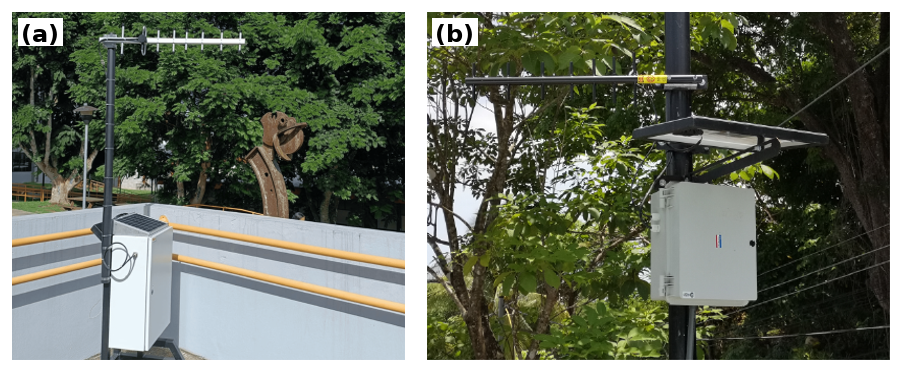
\includegraphics[width=0.85\textwidth]{figure-000.png}
\caption{Representative hardware documented for (a) Paso Ancho--Boquerón and (b) Playa Sámara \cite{solorzano2021sistema,oviedo2024desarrollo}.}
\label{fig:hardware}
\end{figure*}

\section{Formalization through MBSE}
The experiences reveal a recurring functional structure: measurement $\rightarrow$ acquisition $\rightarrow$ communication $\rightarrow$ digital service $\rightarrow$ information for the operator. Sensors, controllers, links, platforms, energy arrangements, and the degree of operational support may change.

Here, MBSE provides a conceptual framework for synthesis. ARCADIA refers to the systems-engineering and model-based architecture method documented by Voirin \cite{voirin2018arcadia}. The generic ARCADIA architecture was developed in the ISSE 2025 work \cite{arguedas2025towards}. This article uses its separation between operational needs, logical functions, and physical implementations to interpret the three cases. The original reports used their own design approaches, including the function, behavior, structure, and experience classification in Paso Ancho--Boquerón. Their processes are compared retrospectively through the MBSE framework.

That separation makes it possible to move from HTTP to MQTT, from LoRa to LTE, from an ultrasonic sensor to 4--20~mA, or from an external platform to a managed platform without losing the system logic.

\section{Resulting Modular Architecture}
The resulting modular architecture provides a configurable foundation whose components can be selected for each site. Each deployment requires specifications and verification criteria for data acquisition, local validation, energy, communication, ingestion, storage, visualization, notification, backup, and system health.

\subsection{Field Node}
The field node interacts with the hydraulic infrastructure: it may measure level with an ultrasonic sensor, read a 4--20~mA sensor, acquire Octave registers through Modbus, or incorporate other sensors. Its stable function is to transform physical variables into time-stamped data, apply basic validations, and prepare communication. Calibration, environmental protection, consumption, and maintainability must be designed from the outset.

\subsection{Energy and Communication}
Energy and communication depend on the site. Las Juntas combined solar power with cellular communication. Sámara used solar-powered LoRa devices and a gateway, and Paso Ancho--Boquerón integrated a solar-powered industrial node with LoRa and WiFi communication. These elements must therefore be treated as replaceable modules with verifiable requirements for frequency, availability, autonomy, recovery, consumption, and environmental protection.

\subsection{Digital Services and Operation}
The digital layer must store data, make them accessible, and convert them into operational information. Web visualization, IoT services, cloud services, dashboards, notifications, backups, and access control are instances of general functions: persistence, query, visualization, alerting, analysis, and maintenance.

\section{Current Application in Paso Ancho}
The current Paso Ancho application adapts the modular architecture for a deployment under development \cite{deltalabo2026repo}. The mission-definition documentation lists requirements for mobile monitoring, overflow and insufficient-supply alerts, acquisition from an Octave meter and a level sensor, operation without fixed power or Internet, environmental protection, maintainability, availability, and cybersecurity.

The reviewed ESP32 firmware initializes RS-485, reads flow and volume from the Octave meter through Modbus, reads an analog height input, scales it to 0--5~m, and emits results through a serial port. The SIM7600 wrapper is commented out. LTE transmission, remote upload, and end-to-end integration remain pending in this version. The sensor interface also requires resolution: the documentation describes a 24~V One-Wire depth sensor, whereas the firmware implements an analog input. The deployed version will need a documented and verified physical, electrical, and data interface.

The remaining artifacts describe design requirements and planned tests. Verification of the remote platform, cybersecurity, availability, backups, node health, notifications, and end-to-end operation remains future work. Communication choices will need to satisfy the requirement of transferring data from a site without fixed Internet. Performance claims will require interface control documents, the deployed firmware and configuration, raw data, and test protocols.

\section{Discussion: Lessons Learned and Transferability}
The three cases show how prototyping addressed design uncertainty under different site constraints. Las Juntas compared component and communication alternatives, then revised the modem and power-switching arrangement. Sámara used meter tests to revise pulse interpretation and developed a common circuit for distributed nodes. Paso Ancho--Boquerón organized requirements by function, behavior, structure, and experience, and resolved industrial-interface configuration through staged tests. Across the reports, requirements definition, component selection, integration, testing, and revision formed a recurring design process. This sequence suggests that digitalization of an ASADA can advance incrementally, beginning with information availability and adding capabilities as site constraints become clearer.

One important lesson is the value of incremental modernization. Preserving Octave meters and other functional assets can reduce infrastructure replacement, initial costs, and operational disruption. However, this strategy also shifts complexity toward acquisition interfaces, protocol interpretation, calibration, and fault diagnosis. Interoperability therefore requires compatible connections and preservation of data meaning, quality, and traceability along the entire chain.

The comparison also shows that no universal option exists for energy and communication. LoRa, cellular communication, WiFi, and different solar-power configurations respond to specific conditions of coverage, distance, electrical availability, consumption, and maintenance. Technology selection should follow verifiable requirements for measurement frequency, autonomy, availability, fault recovery, and environmental protection. Modularity offers an advantage only when interfaces and verification criteria are defined with sufficient precision.

From this perspective, MBSE functions as a framework for relating operational needs, system functions, and physical implementations. In this article, it supports synthesis and transfer using the architecture presented at ISSE 2025 as a reference. Its utility lies in allowing an ASADA to select a combination of sensors, controllers, communications, and digital services without losing the common functional structure identified in the analyzed cases.

The scope of the analysis corresponds to three experiences developed in Costa Rican ASADAS and does not aim to represent all community water organizations in the country. The comparison applies common extraction categories to reports with different design methods, testing conditions, and levels of detail. Las Juntas documents explicit alternative comparisons, Sámara develops subsystem-specific designs and tests, and Paso Ancho--Boquerón structures requirements and integration around a replicable node. A shared extraction scheme preserves these differences. The reported precision, communication, energy, and operational results remain unsuitable for direct numerical comparison. In addition, there is still no evidence of prolonged operation that would allow availability, energy autonomy, maintenance, operator acceptance, or effects on water losses and service continuity to be quantified. These aspects should be evaluated through future field deployments with common metrics.

\section{Future Work: Operational Evaluation}
Future work will focus on completing integration of the current architecture and evaluating it under representative operating conditions. The first stage will verify the acquisition, communication, storage, visualization, notification, and node-status monitoring chain. A sustained deployment will then observe system behavior under variations in connectivity, energy, sensors, and environmental conditions.

The evaluation should quantify data availability, recovery from communication failures, energy autonomy, measurement plausibility, alert behavior, maintenance interventions, and operator acceptance. These results will make it possible to determine which functions and modules can be transferred directly to other ASADAS and which require adaptation. Advanced functions, such as water-loss analysis and supervisory control, should be evaluated only after the reliability of the basic monitoring infrastructure has been demonstrated.

\section{Conclusion}
This work synthesized three digitalization experiences developed for Costa Rican ASADAS: Las Juntas de Abangares, Playa Sámara, and Paso Ancho--Boquerón. The comparative analysis indicates that, although the technologies differed, needs related to remote observability, interoperability with existing infrastructure, communication from isolated sites, energy autonomy, and operational support recurred across the cases.

The main contribution of the synthesis is to distinguish functions that can be reused from components that must be adapted to each aqueduct. In this framework, MBSE is used as a conceptual tool to relate operational needs, system functions, and physical implementations, complementing the architecture work published at ISSE 2025. The available evidence supports the initial feasibility of the prototypes. Claims of sustained performance, reduced water losses, improved service continuity, or generalized transferability require prolonged field tests that evaluate availability, energy autonomy, communication, alerts, maintenance, and security.

\section*{Statement on the Use of Artificial Intelligence}
The authors declare that an OpenAI language model was used as an auxiliary tool for language editing, technical wording review, bibliographic consistency checking, and LaTeX formatting. The tool was not used to generate research data, create or manipulate figures, perform measurements, conduct analyses, or produce results. All sources, interpretations, conclusions, and final manuscript content were reviewed, verified, and approved by the authors, who take full responsibility for the work.

\begin{thebibliography}{12}

\bibitem{arnell2023making}
M. Arnell, M. Miltell, and G. Olsson, ``Making Waves: A Vision for Digital Water Utilities,'' \emph{Water Research X}, vol.~19, p. 100170, 2023, doi: 10.1016/j.wroa.2023.100170.

\bibitem{zulkifli2022iot}
C. Z. Zulkifli \emph{et al.}, ``IoT-Based Water Monitoring Systems: A Systematic Review,'' \emph{Water}, vol.~14, no.~22, p. 3621, 2022, doi: 10.3390/w14223621.

\bibitem{velayudhan2022iot}
N. K. Velayudhan, P. Pradeep, S. N. Rao, A. R. Devidas, and M. V. Ramesh, ``IoT-Enabled Water Distribution Systems---A Comparative Technological Review,'' \emph{IEEE Access}, vol.~10, pp. 101042--101070, 2022, doi: 10.1109/ACCESS.2022.3208142.

\bibitem{direccion2025asadas}
Dirección de Agua de Costa Rica, ``ASADAS,'' 2025. [Online]. Available: \url{https://da.go.cr/asadas/}

\bibitem{soto2016situacion}
S. M. Soto-Córdoba, L. Gaviria-Montoya, and M. Pino-Gómez, ``Situación de la gestión del agua potable en las zonas rurales de la provincia de Cartago, Costa Rica,'' [in Spanish], \emph{Revista Tecnología en Marcha}, vol.~29, no.~8, pp. 67--76, 2016, doi: 10.18845/tm.v29i8.2986.

\bibitem{gaviria2020risk}
L. Gaviria-Montoya, M. Pino-Gómez, and S. M. Soto-Córdoba, ``Risk Associated with the Water Infrastructure in Rural Water Suppliers in Turrialba, Cartago, Costa Rica,'' \emph{Sustainable Water Resources Management}, vol.~6, art. no.~56, 2020, doi: 10.1007/s40899-020-00410-x.

\bibitem{chavarria2021implementacion}
Y. J. Chavarría Castro, ``Implementación de un sistema prototipo para el monitoreo de la variación de nivel de líquido, en una ASADA ubicada en la comunidad de las Juntas de Abangares,'' [in Spanish], Final graduation project, Escuela de Ingeniería Electrónica, Instituto Tecnológico de Costa Rica, Costa Rica, 2021. [Online]. Available: \url{https://hdl.handle.net/2238/15115}

\bibitem{solorzano2021sistema}
S. Solórzano Alfaro, ``Sistema de control y monitoreo hídrico, basado en LoRaWAN, para el acueducto principal de la Asociación Administradora del Acueducto Rural de Playa Sámara de Nicoya,'' [in Spanish], Specialization practice report, Escuela de Ingeniería Electromecánica, Instituto Tecnológico de Costa Rica, Costa Rica, 2021. [Online]. Available: \url{https://hdl.handle.net/2238/13234}

\bibitem{oviedo2024desarrollo}
A. Oviedo Muñoz, ``Desarrollo de un prototipo para recopilación y monitoreo remoto de datos hídricos de los tanques, basado en dispositivos IoT, en la ASADA Paso Ancho y Boquerón,'' [in Spanish], Specialization practice report, Escuela de Ingeniería Electromecánica, Instituto Tecnológico de Costa Rica, Cartago, Costa Rica, 2024. [Online]. Available: \url{https://github.com/DeltaLabo/ASADA_Paso_Ancho/blob/b791b87/TFG_Alejandra.pdf}

\bibitem{arguedas2025towards}
A. J. Arguedas-Rodríguez, M. J. Angulo-Campos, J. J. Montero-Jiménez, and J. J. Rojas-Hernández, ``Towards a Modular IoT System Architecture for Rural Aqueducts Using Model-Based Systems Engineering,'' in \emph{2025 IEEE International Symposium on Systems Engineering (ISSE)}, 2025, doi: 10.1109/ISSE65546.2025.11369985.

\bibitem{deltalabo2026repo}
DeltaLabo, ``ASADA\_Paso\_Ancho: documentation and code for the design under development,'' GitHub, 2026, reviewed revision b791b87. [Online]. Available: \url{https://github.com/DeltaLabo/ASADA_Paso_Ancho/tree/b791b87}

\bibitem{voirin2018arcadia}
J.-L. Voirin, \emph{Model-Based System and Architecture Engineering with the Arcadia Method}. ISTE Press--Elsevier, 2018, doi: 10.1016/C2016-0-00862-8.

\end{thebibliography}

\end{document}
